\documentclass[letterpaper,11pt]{article}

\usepackage{geometry, pslatex, fancyhdr, graphicx}
\usepackage{amsmath,amsthm,amssymb,scrextend}
\usepackage{multicol}
\usepackage{tabularx}
\usepackage[makeroom]{cancel}
\usepackage{color}
\geometry{ margin = 1.0in }

%%% TODO modify these variables as per your homework %%%
\def\homeworknum{2}
\def\myname{Harshit Jain}
\def\myuserid{hmj5262}
%%%%

\pagestyle{fancy}
\lhead{{\bf CMPSC 461 Spring 2023}}
\chead{{\bf Assignment~\homeworknum}}
\rhead{{\bf \today}}
\let\newproof\proof
\renewenvironment{proof}{\begin{addmargin}[1em]{0em}\begin{newproof}}{\end{newproof}\end{addmargin}\qed}

\newcounter{problemid}
\stepcounter{problemid}
\def\newproblem{\clearpage\newpage{\bf Problem~\arabic{problemid}\stepcounter{problemid}}\hfill\par}

\setlength\parindent{0em} 
\setlength\parskip{8pt}
\setlength{\fboxsep}{6pt}


\begin{document}

\framebox[\textwidth]{
	\parbox{0.96\textwidth}{
		\parbox{0.12\textwidth}{\bf Name:}\parbox{0.6\textwidth}{\myname}\\
		\parbox{0.12\textwidth}{\bf User ID:}\parbox{0.6\textwidth}{\myuserid}
	}
}
%% your solutions %%%


% PROBLEM 1
\newproblem 
\begin{enumerate}
    \item Code A and Code B differ in terms of the scope of the variable "count".
    
    In Code A, the variable "count" is declared as a static variable inside the function "globalCounter". This means that the variable "count" retains its value between function calls, and its scope is limited to the function "globalCounter".
    
    In Code B, the variable "count" is declared as a local variable inside the function "globalCounter", which means that its value is reset to 0 each time the function is called and its scope is limited to the function "globalCounter".

    \item The output of Code A will be$:$
    
        count $= 1$
        
        count $= 2$
        
        count $= 3$
        
        count $= 4$
        
        count $= 5$

        The output of Code B will be$:$

        count $= 0$
        
        count $= 0$
        
        count $= 0$

\end{enumerate}



% PROBLEM 2
\newproblem 
\begin{enumerate}
    
    \item Yes, C is a statically scoped language. In a statically scoped language, the scope of a variable is determined at compile time and remains fixed throughout the program's execution. In other words, the scope of a variable is the part of the program where it is accessible and can be used.
    
    In C, the scope of a variable is determined by its location within the source code and the scope rules specified by its declaration.
    
    \item 
    \begin{enumerate}
        
        \item The scope of a static local variable is the block scope. The lifetime of a static local variable is the entire program.
        
        \item The scope of a static global variable is the file scope. The lifetime of a static global variable is the entire program.
        
        \item The scope of a non-static local variable is limited to the block - block scope. The lifetime of a non-static local variable is limited to the duration of a function call.
        
        \item The scope of a non-static global variable is the file scope. The lifetime of a non-static global variable is the entire program.

    \end{enumerate}
\end{enumerate}




% PROBLEM 3
\newproblem 
\begin{enumerate}

    \item 
    
    Global Scope:
    
    \begin{tabularx}{0.8\textwidth} { 
        | >{\raggedright\arraybackslash}X 
        | >{\centering\arraybackslash}X 
        | >{\raggedleft\arraybackslash}X | }
        \hline
        \textbf{Name} & \textbf{Type} \\
        \hline
        x & int \\
        \hline
    \end{tabularx}
    
    first():

    \begin{tabularx}{0.8\textwidth} { 
        | >{\raggedright\arraybackslash}X 
        | >{\centering\arraybackslash}X 
        | >{\raggedleft\arraybackslash}X | }
        \hline
        \textbf{Name} & \textbf{Type} \\
        \hline
        x & int \\
        \hline
    \end{tabularx}
    
    second():

    \begin{tabularx}{0.8\textwidth} { 
        | >{\raggedright\arraybackslash}X 
        | >{\centering\arraybackslash}X 
        | >{\raggedleft\arraybackslash}X | }
        \hline
        \textbf{Name} & \textbf{Type} \\
        \hline
        x & int \\
        \hline
    \end{tabularx}
    
    third():

    \begin{tabularx}{0.8\textwidth} { 
        | >{\raggedright\arraybackslash}X 
        | >{\centering\arraybackslash}X 
        | >{\raggedleft\arraybackslash}X | }
        \hline
        \textbf{Name} & \textbf{Type} \\
        \hline
        x & int \\
        \hline
    \end{tabularx}
    
    Code block within third():

    \begin{tabularx}{0.8\textwidth} { 
        | >{\raggedright\arraybackslash}X 
        | >{\centering\arraybackslash}X 
        | >{\raggedleft\arraybackslash}X | }
        \hline
        \textbf{Name} & \textbf{Type} \\
        \hline
        x & int \\
        \hline
    \end{tabularx}

    \item 
    If the language uses static scoping rules, the expected output from the print statement would be \textbf{25} and \textbf{10}.
    
    When the $third$ function is called from the $first$ function, the $x$ parameter in the $third$ function is assigned the value of $x$ from the $first$ function, which is $25$. The $x$ in the global scope remains unchanged at $10$. When the $second$ function is called within the code block in $third$, it will use the value of $x$ from the global scope, which is $10$.

    \item If the language uses dynamic scoping rules, the expected output from the print statement would be \textbf{30} and \textbf{30}.
    
    Dynamic scoping means that the value of a variable is determined by the most recent call in the call chain. In this case, the $x$ in the code block within $third$ is assigned the value of $30$, which would be used by both $third$ and $second$, since $second$ is called within $third$.

\end{enumerate}


% PROBLEM 4
\newproblem
    
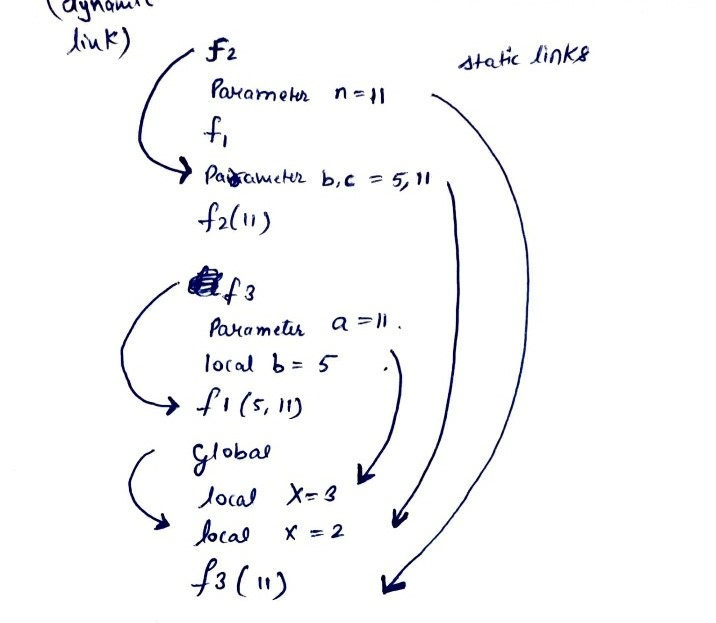
\includegraphics[scale = 0.60]{4.1} 


% PROBLEM 5
\newproblem 
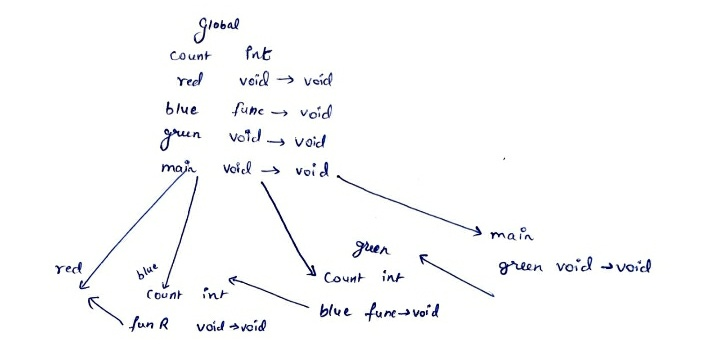
\includegraphics[scale = 0.60]{5.1}
\begin{enumerate}

    \item blue $0$, green $0$, counter value $1$
        
        \begin{enumerate}
            \item Global is the top level thus edits global count
        \end{enumerate}
    
    \item blue $1$, green $0$ , counter value $0$
        
        \begin{enumerate}
            \item This is because red goes back one later according to the table and thus edits blues local count
        \end{enumerate}
    
    \item blue $0$, green $1$, counter value $0$
        
        \begin{enumerate}
            \item This is because red is passed through at green, editing greens local count according to the table (blue accepts red)
        \end{enumerate}

\end{enumerate}

% PROBLEM 6
\newproblem
\begin{enumerate}

    \item \textbf{Storage Allocation}
    
        \begin{enumerate}

            \item $A$ is a static object therefore stored on static
            
            \item $C$ is assigned to the object created using new therefore stored on heap
            
            \item $D$ is neither static nor using new therefore stored on stack
            
            \item $B$ is assigned to the $C$ created in foo which is on heap therefore $B$ points to heap
            
            \item $C$ also points to something on heap

        \end{enumerate}

    \item \textbf{Lifetime}

        \begin{enumerate}

            \item $A:$ Entire program
            
            \item $C:$ When it gets deleted  $13 14 15 6 7$
            
            \item $D:$ It is on stack therefore it's lifetime ends when it goes out of scope  $14 15$
        
        \end{enumerate}

\end{enumerate}

\end{document}